\documentclass{article}
\usepackage[T1]{fontenc}
\usepackage{lmodern}
\usepackage{graphicx}
\usepackage{amsmath,amssymb}
\usepackage[a4paper,margin=2cm]{geometry}
\usepackage[absolute,overlay]{textpos}
\setlength{\TPHorizModule}{1mm}
\setlength{\TPVertModule}{1mm}
\usepackage[indonesian]{babel}
\usepackage{hyperref}
\setlength{\emergencystretch}{2em}
% unit: Halaman 76

\begin{document}

% === Halaman 76 (llm) ===

\vspace{60mm}

\textbf{Inisialisasi:}
\begin{itemize}
    \item Masukkan 80-bit \textit{initialization vector} (IV) ke dalam A
    \item Masukkan 80-bit kunci ke dalam B
    \item Set $c_{109}, c_{110}, c_{111} = 1$, sedangkan bit lainnya 0
\end{itemize}

\textbf{Pemanasan (\textit{warming-up}):}
\begin{itemize}
    \item Detak (\textit{clock}) NLFSR $4 \times 288 = 1152$ kali tanpa menghasilkan luaran (luaran diabaikan)
    \item Tujuannya adalah melakukan pencampuran kunci/IV sehingga pengaruh kunci dan IV tersebar ke seluruh register
\end{itemize}

\textbf{Encryption:}
\begin{itemize}
    \item XOR-kan ketiga buah luaran NLFSR untuk membangkitkan kunci-alir $s_i$
    \item XOR-kan $s_i$ dengan bit plainteks $p_i$
\end{itemize}

% deskripsi: Diagram blok arsitektur kriptografi yang menunjukkan tiga register NLFSR (A, B, C) dengan jalur feedback, XOR gates, dan output key stream s_i.
% bbox normalisasi: [0.4800, 0.1000, 0.9300, 0.4400]
\begin{textblock*}{94.50mm}(100.80mm,29.70mm)
\noindent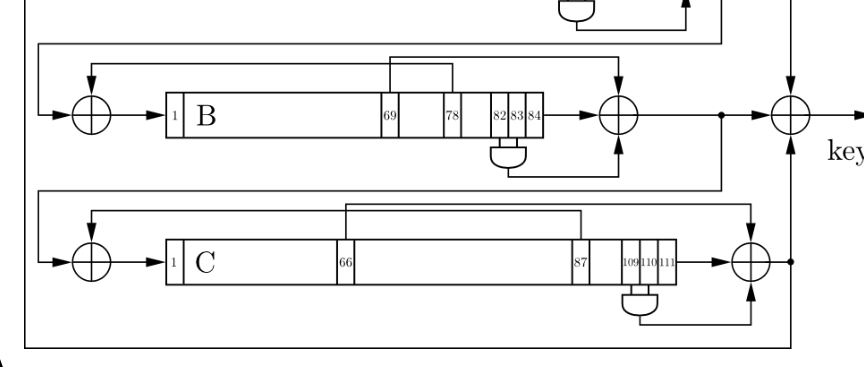
\includegraphics[width=94.50mm,height=100.98mm]{../../images/llm/page_076_img_01.png}%
\end{textblock*}

\end{document}
